\section{Promises}

Javascript/Typescript ist grundsätzlich eine sequenziell ausführende Skriptsprache. Das heißt,  dass zwei Bits eines Skripts nicht im gleichen Augenblick ausführbar sind. Sie müssen nacheinander ausgeführt werden. Im Browser können neben Javascript, auch CSS aktualisiert oder der Einfluss von außen, wie User-Interaktionen, ausgeführt werden. Und jede Operation verlangsamt die Andere. Um dem entgegenzuwirken hat man in dieser Arbeit schon das Prinzip der Callbacks gesehen. Dank der Rückruffunktionen ist die Ausführung dieser Sprache in asynchron möglich. Mit Callbacks kann man beispielsweise User-Events gut steuern. Ein User drückt auf die Enter-Taste und nach dem Event wird eine Funktionalität aufgerufen. Diese können in multiplen Ausführungen geschehen. Sollten jedoch Events von anderen Ressourcen abhängen, wie z.B. das Event darf erst eine Funktionalität \glqq{}feuern\grqq{} wenn das Bild im Browser geladen ist. Und sollte das Bild nicht geladen sein, sollte eine entsprechende Fehlermeldung angezeigt werden. Der Code hierfür würde wie folgt aussehen:

\begin{figure}[H]
\begin{lstlisting}
img1.callThisIfLoadedOrWhenLoaded(/** Callback 1 **/ () => {
  // Add Eventlistener to change the background
}).orIfFailedCallThis(/** Callback 2 **/ () => {
  // Show error msg for the user
});
\end{lstlisting}
\end{figure}

\noindent
Und genau das bieten \textbf{Promises} in einer übersichtlichen Form.

\begin{figure}[H]
\begin{lstlisting}
img1.ready().then(() => {
  // Add Eventlistener to change the background
}).catch(() => {
  // Show error msg for the user
});
\end{lstlisting}
\caption{Beispiel inspiriert von Google-Developer-Docs \cite{callback-vs-promises}}
\end{figure}

\noindent
Im Gegensatz zu Callbacks sind Promises an einer einzelner asynchronen erfolgreichen/fehlgeschlagenen Interaktion interessiert und weniger wann die Interaktion stattgefunden hat. Promises sind danach gerichtet wie man mit Ergebnis der Interaktion umgeht. 
Doch was genau sind Promises? \\

\subsection{Funktionsweise}

\noindent
Sie \textit{(\glqq{}Promises\grqq{} zu deutsch: Versprechen)} in Javascript verhalten sich ähnlich wie im echten Leben. Die Definition aus dem Wörterbuch ist: Das Versprechen ist eine einseitige Zusage über eine zukünftige Handlung oder ein zukünftiges Ereignis. \cite{versprechen} \\

\noindent
Das heißt:

\begin{enumerate}
    \item Ein Versprechen ist eine Absicherung, dass etwas gemacht wird. Unabhängig davon, ob das Versprechen sich selbst oder von einer anderen Partei gegeben wird.
    
    \item Ein Versprechen kann eingehalten oder gebrochen werden.
    
    \item Wurde ein Versprechen nicht eingehalten, möchte man den Grund für die Nichteinhaltung wissen um darauffolgend zu handeln.
    
    \item Beim Zeitpunkt eines Versprechens hat man nur die Absicherung. Man kann damit erstmal noch nichts anfangen. Es kann nur geplant werden was nach dem Einhalten des Versprechens gemacht wird. Dementsprechend kann man auch Maßnahmen setzen beim Nichteinhalten dieser Absicherung.
    
\end{enumerate}

\noindent
Und genauso ist das Verhalten der Promises in Javascript. Dabei gibt es zwei grundlegende Prinzipien der Promises, die zu Verstehen sind: Das \textbf{Erstellen von Promises} und das \textbf{Verarbeiten von Promises}.

\subsubsection{Erstellen eines Promises}

\begin{figure}[H]
\begin{lstlisting}
new Promise( /* executor */ (resolve, reject)  => { ... } );
\end{lstlisting}
\caption{Erzeugung einer neuen Promise-Instanz}
\end{figure}

Der Konstruktor nimmt eine Funktion als Eingangsparameter. Diese Funktion wird auch \textbf{Executor} genannt.\cite{promise-executor} Der Executor akzeptiert zwei Parameter \textbf{resolve} und \textbf{reject}. Innerhalb dieser Funktion wird eine asynchrone Operation initiiert (z.B. Das suchen einer Datei, eine Datenbankabfrage etc.). Wurde diese asynchrone Operation erfolgreich ausgeführt, ruft der Promise-Konstruktor die resolve Funktion mit dem entsprechendem Ergebnis auf. Anders, bei einem unerwartetem Fehler, ruft der Konstruktor die reject Funktion mit der jeweiligen Fehlernachricht auf. Zur Einführung ein einfaches Beispiel:\\

\noindent
Vor dem Ausführen des Beispiels muss folgend konfiguriert werden:

 \begin{center}
     Promises-vs.-Observables$\,\to\,$ webpack.config.js
 \end{center}

\begin{figure}[H]
\begin{lstlisting}
module.exports = {
    mode: 'development',
    entry: './src/modules/modules/introduction.ts',
    ...
}
\end{lstlisting}
\end{figure}

\begin{figure}[H]
\begin{lstlisting}
const keepsHisWord = true;
const promise = new Promise((resolve, reject) => {
    if (keepsHisWord) {
        resolve('Promises kept!');
    } else {
        reject('Promise NOT kept!');
    }
});

console.log(promise);
\end{lstlisting}
\end{figure}

\noindent
Dieser Promise löst sich auf Anhieb auf und der Status gelangt in den resolved Zustand, da die abhängige boolean-Variable vorher auf true gesetzt wurde. Umgekehrt, würde die boolean Variable auf false gesetzt werden, würde der Status rejected entsprechen. Der Anfangsstatus des Promise wird im nächsten Beispiel verdeutlicht:

\begin{figure}[H]
\centering
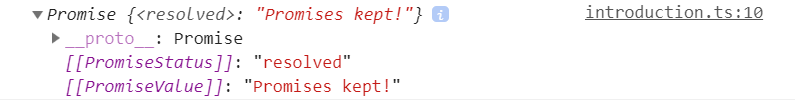
\includegraphics{promise-beispiel-1}
\caption{Promises haben einen Status und einen Wert}
\end{figure}

\begin{figure}[H]
\begin{lstlisting}
export interface FakeHttpResponse {
    code: string;
    message: string;
}

const scndPromise = new Promise<FakeHttpResponse>((resolve, reject) => {
    setTimeout(() => {
        resolve({
            code: '200',
            message: 'Promise kept!'
        });
    }, 10 * 1000);
});

console.log(scndPromise);
setTimeout(() => console.log(scndPromise), 10 * 1000);
\end{lstlisting}
\end{figure}

\noindent
Im oberen Beispiel wird der Promise vorbehaltlos nach zehn Sekunden aufgelöst, solange ist der Status ausstehend. Nachdem der Promise aufgelöst wurde, werden Status und Wert aktualisiert. Dabei können nicht nur primitive Typen wie number, boolean oder string zurückgegeben werden, sondern auch generierte und komplexe Typen. Mit anderen Worten: Promises sind generisch.
\subsubsection{Zustände}

\begin{figure}[H]
\centering
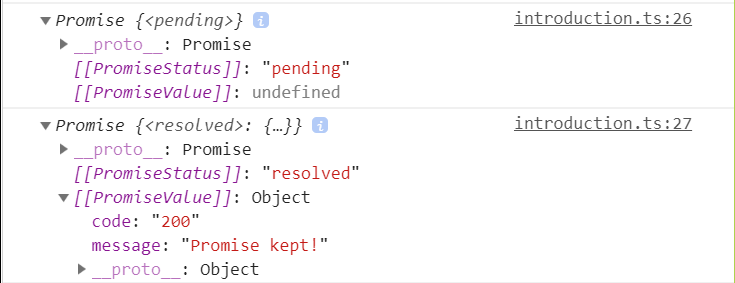
\includegraphics{promise-beispiel-2}
\caption{Promise hat anfangs den Status \glqq{}ausstehend\grqq{}}
\end{figure}

\begin{enumerate} 
\item Pending Ausgang des Promises ist noch(!) ungewiss
\item Resolved Die Aktion die zum Promise verlief schlug ein
\item Rejected Die Aktion die zum Promise verlief schlug fehl
\item Settled - Die Aktion ist entweder fehlgeschlagen oder eingeschlagen
\end{enumerate}

\subsection{Operatoren}

\begin{enumerate} 
\item Promise.all()
\item Promise.race() 
\item Promise.reject()
\end{enumerate}

\subsection{Promise Verkettung}
**Anwendungsbeispiel anzeigen**

\subsection{Async await}
**Funktionsweise und Vorteile**

\subsubsection{Anwendungsfall}

\begin{enumerate} 
\item Source code Beispiel zeigen mit async await
\item Wie wandle ich z.b. eine verkettete (unlesbare) Promise-Verkettung in async await um 
\item Gegenüberstellung
\item Browser kompatibilität
\end{enumerate}


